Para descomponer un número en factores primos solo basta con seguir la idea aprendida en enseñanzas anteriores ejemplo:

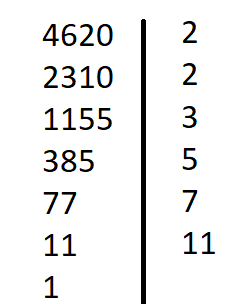
\includegraphics[scale=0.4]{img/descomposicion_primos}

En esta caso $4620=2^{2}*3^{1}*5^{1}*7^{1}*11^{1}$


\subsection{Probando divisiones}

Este es el algoritmo más básico para encontrar una factorización prima.

Dividimos por cada posible divisor $d$. Podemos notar que es imposible que todos los factores primos 
de un número compuesto $n$ son más grandes que $\sqrt{n}$. Por lo tanto, solo necesitamos probar los 
divisores $2 \le d \le \sqrt{n}$ , lo que nos da la factorización prima en $O(\sqrt{n})$. (Este es un 
tiempo pseudo-polinómico , es decir, polinomial en el valor de la entrada pero exponencial en el 
número de bits de la entrada).

El divisor más pequeño tiene que ser un número primo. Eliminamos el factor del número y repetimos el 
proceso. Si no podemos encontrar ningún divisor en el rango $[2; \sqrt{n}]$, entonces el número en sí 
tiene que ser primo.

\subsubsection{Factorización de ruedas}

Esta es una optimización de la idea anterior. La idea es la siguiente. Una vez que sabemos que el número no es divisible por 2, no necesitamos verificar todos los demás números pares. Esto nos deja solo con $50\%$ de los números a comprobar. Después de marcar 2, simplemente podemos comenzar con 3 y omitir cualquier otro número.

Este método se puede ampliar. Si el número no es divisible por 3, también podemos ignorar todos los 
demás múltiplos de 3 en los cálculos futuros. Así que solo tenemos que comprobar los números. $5, 7, 
11, 13, 17, 19, 23, \dots$ . Podemos observar un patrón de estos números restantes. Tenemos que 
comprobar todos los números con $d \bmod 6 = 1$ y $d\bmod 6 = 5$. Así que esto nos deja con sólo $33,3\%$ porcentaje de los números a verificar. Podemos implementar esto verificando primero los 
números primos 2 y 3, y luego comenzar a verificar con 5 y, alternativamente, omitir 1 o 3 números.

Si ampliamos esto más con más números primos, incluso podemos llegar a mejores porcentajes. Sin embargo, también las listas de saltos serán mucho más grandes.

\subsection{Primos precalculados}


\subsubsection{Factorización de N}

Una buena manera de verificar es precalcular todos los números primos con la criba de Eratóstenes hasta $\sqrt{N}$ y probarlos individualmente.

Para un factor primo $p$ de $N$, la multiplicidad de $p$ es el máximo exponente $a$ para el cual $p^a$ es un divisor de $N$. La factorización de un número entero es una lista de los factores primos de ese número, junto con su multiplicidad. El Teorema fundamental de la Aritmética establece que todo número entero positivo tiene una factorización de primos única.

\subsubsection{Factorización de N!}

Que pasa si ahora queremos descomponer N! la idea básica seria iterar desde 1 hasta N e ir descomponiendo cada número acumulando las potencias o hallar N! y luego descomponerlo, pero esto tendría una complejidad de O($N* \sqrt{N}$) el cual sería muy costoso para valores muy grandes de N. Analicemos la siguiente idea:

10!=1*2*3*4*5*6*7*8*9*10 Necesitamos hallar cuantos 2 hay.

\begin{tabular}{|c|c|c|c|c|c|c|c|c|c|c|c|}
	\hline 
	10!& 1 & 2 & 3 & 4 & 5 & 6 & 7 & 8 & 9 & 10 & total \\ 
	\hline 
	Descomposición de n1& 1 & 2 & 3 & 2$^{2}$ & 5 & 2*3 & 7 & 2$^{3}$ & 3$^{2}$ & 2*5 &  \\ 
	\hline 
	Primo 2& 0 & 1 & 0 & 2 & 0 & 1 & 0 & 3 & 0 & 1 & 8 \\ 
	\hline 
	Primo 3& 0 & 0 & 1 & 0 & 0 & 1 & 0 & 0 & 2 & 0 & 4 \\ 
	\hline 
\end{tabular} 

\hspace{0.5em}

Para el caso del 2 seria todos los múltiplos de 2 hasta N ejemplo para 10 hay 5 que seria 10/2 luego todos los múltiplos de 4 hasta N que sería N/4 y así hasta que la potencia de 2 sea mayor que N la suma de estos seria el exponente de la potencia de 2 luego de descomponer N!, en  este caso sería 2$^{10/2+10/4+10/8}$=2$^{5+2+1}$=2$^{8}$ y este sería el procedimiento para todos los primos hasta N.

\subsection{Método de factorización de Fermat}

Podemos escribir un número compuesto impar $n = p \cdot q$ como la diferencia de dos cuadrados $n = a^2 - b^2$:

$$n = \left(\frac{p + q}{2}\right)^2 - \left(\frac{p - q}{2}\right)^2$$

El método de factorización de Fermat trata de explotar el hecho, adivinando el primer cuadrado $a^2$ y compruebe si la parte restante $b^2 = a^2 - n$ también es un número cuadrado. Si es así, entonces hemos encontrado los factores $a - b$ y $a + b$ de $n$.

\subsection{Método de Pollard's \emph{p-1}}

Es muy probable que al menos un factor de un número sea $B$-powersmooth para pequeños $B$. $B$-powersmooth significa que cada potencia principal $d^k$ que divide $p-1$ es como mucho $B$. Por 
ejemplo, la descomposición en factores primos de $4817191$ es $1303 \cdot 3697$. Y los factores son $31$-poderoso y suave $16$-powersmooth respetablemente, porque $1303 - 1 = 2 \cdot 3 \cdot 7 \cdot 
31$ y $3697 - 1 = 2^4 \cdot 3 \cdot 7 \cdot 11$. En 1974, John Pollard inventó un método para extraer $B$-powersmooth factores de un número compuesto.

La idea proviene del pequeño teorema de Fermat . Sea una factorización de $n$ ser $n = p \cdot q$. Dice que si $a$ es coprimo de $p$, se cumple el siguiente enunciado:

$$ a^{p - 1} \equiv 1 \pmod{p} $$

Esto también significa que

$$ a^{(p - 1)^k} \equiv a^{k \cdot (p - 1)} \equiv 1 \pmod{p}. $$

Así que para cualquier $M$ con $p - 1 ~|~ M$ lo sabemos $a^M \equiv 1$. Esto significa que $a^M - 1 = p \cdot r$ , y por eso también $p ~|~ \gcd(a^M - 1, n)$.

Por lo tanto, si $p-1$ por un factor $p$ de $n$ divide $M$, podemos extraer un factor usando el algoritmo de Euclides.

Está claro que los más pequeños $M$ que es múltiplo de cada $B$-el número de powersoft es $\text{lcm}(1,~2~,3~,4~,~\dots,~B)$. O alternativamente:

$$M = \prod_{\text{prime } q \le B} q^{\lfloor \log_q B \rfloor}$$

Aviso, si $p-1$ divide $M$ para todos los factores primos $p$ de $n$, entonces $\gcd(a^M - 1, n)$ solo será $n$. En este caso no recibimos un factor. Por lo 
tanto, intentaremos realizar la $\gcd$ varias veces, mientras calculamos $M$.

Algunos números compuestos no tienen $B$-powersmooth factores para pequeños $B$. Por ejemplo, los factores del número compuesto $100~000~000~000~000~493 = 763~013 \cdot 131~059~365~961$ son $190~753$-poderoso y suave $1~092~161~383$-poderoso. Tendríamos que elegir $B >= 190~753$ para factorizar el número.

\subsection{Algoritmo rho de Pollard}
Otro algoritmo de factorización de John Pollard.

Sea la factorización prima de un número $n = pq$. El algoritmo analiza una secuencia pseudoaleatoria 
$\{x_i\} = \{x_0,~f(x_0),~f(f(x_0)),~\dots\}$ dónde $f$ es una función polinomial, generalmente
$f(x) = (x^2 + c) \bmod n$ se elige con $c = 1$.

En realidad no estamos muy interesados en la secuancia  $\{x_i\}$, estamos más interesados en la
secuencia $\{x_i \bmod p\}$. Desde $f$ es una función polinomial y todos los valores están en el 
rango $[0;~p)$ esta secuencia comenzará a circular tarde o temprano. La paradoja del cumpleaños en 
realidad sugiere que el número esperado de elementos es $O(\sqrt{p})$ hasta que comience la 
repetición. Si $p$ es más pequeña que $\sqrt{n}$, la repetición comenzará muy probablemente en 
$O(\sqrt[4]{n})$.

Aquí hay una visualización de tal secuencia $\{x_i \bmod p\}$ con $n = 2206637$, $p = 317$, $x_0 = 2$ y $f(x) = x^2 + 1$. Por la forma de la secuencia se puede ver muy claramente por qué el algoritmo se llama de Pollard $\rho$ algoritmo.

% TODO: \usepackage{graphicx} required
\begin{figure}[h!]
	\centering
	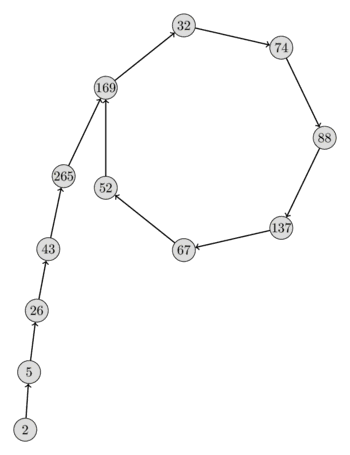
\includegraphics[width=0.3\linewidth]{img/pollard_rho}
	\label{fig:pollardrho}
\end{figure}


Todavía hay una gran pregunta abierta. no sabemos $p$ sin embargo, entonces, ¿cómo podemos discutir sobre la secuencia $\{x_i \bmod p\}$ ?

En realidad es bastante fácil. Hay un ciclo en la secuencia $\{x_i \bmod p\}_{i \le j}$ si y solo si 
hay dos índices $s, t \le j$ tal que $x_s \equiv x_t \bmod p$. Esta ecuación se puede reescribir como 
$x_s - x_t \equiv 0 \bmod p$ que es lo mismo que $p ~|~ \gcd(x_s - x_t, n)$.

Por lo tanto, si encontramos dos índices $s$ y $t$ con $g = \gcd(x_s - x_t, n) > 1$, hemos encontrado un ciclo y también un factor $g$ de $n$. Note que es posible que $g = n$. En este caso, no hemos encontrado un factor adecuado y tenemos que repetir el algoritmo con un parámetro diferente (diferente valor inicial $x_0$, diferente constante $c$ en la función polinomial $f$).

Para encontrar el ciclo, podemos usar cualquier algoritmo común de detección de ciclos.

\subsection{Algoritmo de búsqueda de ciclos de Floyd}

Este algoritmo encuentra un ciclo usando dos punteros. Estos punteros se mueven sobre la secuencia a diferentes velocidades. En cada iteración, el primer puntero avanza al siguiente elemento, pero el segundo puntero avanza dos elementos. No es difícil ver que, si existe un ciclo, el segundo puntero hará al menos un ciclo completo y luego se encontrará con el primer puntero durante los próximos bucles de ciclo. Si la duración del ciclo es $\lambda$ y el $\mu$ es el primer índice en el que comienza el ciclo, entonces el algoritmo se ejecutará en $O(\lambda + \mu)$ tiempo.

Este algoritmo también se conoce como tortuga y el algoritmo de la liebre , basado en el cuento en el que una tortuga (aquí un puntero lento) y una liebre (aquí un puntero más rápido) hacen una carrera.

En realidad, es posible determinar el parámetro $\lambda$ y $\mu$ utilizando este algoritmo (también 
en $O(\lambda + \mu)$ tiempo y $O(1)$ espacio), pero aquí está solo la versión simplificada para 
encontrar el ciclo. El algoritmo y devuelve verdadero tan pronto como detecta un ciclo. Si la 
secuencia no tiene un ciclo, la función nunca se detendrá. Sin embargo, esto no puede suceder durante 
el algoritmo rho de Pollard.

La siguiente tabla muestra los valores de $x$ y $y$ durante el algoritmo de $n = 2206637$, $x_0 = 2$ y $c = 1$.

$ \begin{array}{|l|l|l|l|l|l|} \hline i & x_i \bmod n & x_{2i} \bmod n & x_i \bmod 317 & x_{2i} \bmod 317 & \gcd(x_i - x_{2i}, n) \\ \hline 0 & 2 & 2 & 2 & 2 & - \\ 1 & 5 & 26 & 5 & 26 & 1 \\ 2 & 26 & 458330 & 26 & 265 & 1 \\ 3 & 677 & 1671573 & 43 & 32 & 1 \\ 4 & 458330 & 641379 & 265 & 88 & 1 \\ 5 & 1166412 & 351937 & 169 & 67 & 1 \\ 6 & 1671573 & 1264682 & 32 & 169 & 1 \\ 7 & 2193080 & 2088470 & 74 & 74 & 317 \\ \hline \end{array} $

La implementación utiliza una función multque multiplica dos enteros $\le 10^{18}$ sin desbordamiento utilizando un tipo de GCC \_\_int128para enteros de 128 bits. Si GCC no está disponible, puede usar una idea similar a la exponenciación binaria .

Alternativamente, también puede implementar la multiplicación de Montgomery .

Como ya se ha señalado anteriormente: si $n$ es compuesto y el algoritmo devuelve $n$ como factor, tienes que repetir el procedimiento con diferentes parámetros $x_0$ y $c$. ej., la elección $x_0 = c = 1$ no factorizará $25 = 5 \cdot 5$. El algoritmo simplemente regresará $25$. Sin embargo la elección $x_0 = 1$, $c = 2$ lo factorizará.

\subsection{Algoritmo de Brent}

Brent usa un algoritmo similar al de Floyd. También utiliza dos punteros. Pero en lugar de avanzar los punteros en uno y dos respetablemente, los avanzamos en potencias de dos. Tan pronto como $2^i$ es mayor que $\lambda$ y $\mu$ , encontraremos el ciclo.

La implementación directa utilizando los algoritmos de Brent se puede acelerar al notar que podemos 
omitir los términos $x_l - x_k$ si $k < \frac{3 \cdot l}{2}$. Además, en lugar de realizar la $\gcd$ cálculo en cada paso, multiplicamos los términos y lo hacemos cada pocos pasos y retrocedemos si nos 
sobrepasamos.

La combinación de una división de prueba para números primos pequeños junto con la versión de Brent del algoritmo rho de Pollard creará un algoritmo de factorización muy poderoso.